% Manuscript v5 | 2026-09-28 | v3-final run reported; BDG does not beat its eta=0 arm.
% Build from paper/: pdflatex main; bibtex main; pdflatex main; pdflatex main.
% Previous live sources and PDF: versions/v2_pre_v3_2026-09-27/.
\documentclass{article}
\PassOptionsToPackage{numbers,compress}{natbib}
\usepackage[final,main]{neurips_2026}
\usepackage[utf8]{inputenc}
\usepackage[T1]{fontenc}
\usepackage{amsmath,amssymb,booktabs,graphicx,microtype,url}
\usepackage{algorithm,algpseudocode}
\usepackage{xcolor,tikz}
\usetikzlibrary{arrows.meta,positioning}
\usepackage{hyperref}
\hypersetup{hidelinks,pdftitle={BDG: Batch-Dispersion Guidance for Property-Band Generation},pdfsubject={Manuscript v5, 28 September 2026}}
\newcommand{\pend}{\textcolor{black!60}{\textsf{P}}}
\newcommand{\Fbar}{\bar F}
\newcommand{\Vb}{V_b}
\newcommand{\weff}{w_{\mathrm{eff}}}
\newcommand{\IB}{\mathrm{IB}}
\newcommand{\sg}{\operatorname{stopgrad}}
\title{BDG: Batch-Dispersion Guidance for\\Property-Band Generation}
\author{Bobo Li, Henry Huang, Idea Idehpour, Haimo Fang\\
Department of Computer and Information Science, University of Pennsylvania\\
\small Manuscript v5 \quad 28 September 2026}
\begin{document}
% MAIN_TEXT_START
\maketitle
\begin{abstract}
Property-targeted generation requires samples to fall within a tolerance band around a target while retaining quality and diversity, and one guidance strength moves both a batch's centre and its spread. We introduce Batch-Dispersion Guidance (BDG), an inference-time rule that adjusts the deviation coefficient by the difference between the batch variance of predicted endpoint properties and a specified variance. BDG preserves the target-centering coefficient at the same cost. We study it on QM9 molecular coordinates and DeepFlyBrain DNA sequences. Guidance works and is paid for in chemistry: a plug-in rule raises band coverage over an unguided control at a cost of four points of molecule stability. BDG does not improve on the arm it modifies. Against that plug-in rule, which is BDG at zero gain, twelve contrasts give no gain, three losses and nine ties. What the setpoint does reach is an operating point the strength dial cannot: a batch wider than unguided in six of six cells, where raising the strength only ever narrows it. The ablation establishes the mechanism: at fixed strength, coverage tracks the measured deviation gain at Spearman $0.92$ to $0.99$ across twelve grids, and inverting the setpoint reverses the sign. On the simplex a wider guidance window is worth roughly ten times the rule. Algebraically BDG reweights the plug-in direction through a batch-dependent gain, which bounds what it can reach, and the measurements stay inside that bound.
\end{abstract}

\section{Introduction}
Diffusion and flow matching transport noise to data along different paths \citep{karras2022elucidating,lipman2022flow}, and stochastic interpolants place both under one construction \citep{albergo2025stochastic}, so a matched comparison is not settled in advance.

Gradient guidance steers a frozen generator toward a target \citep{chung2023dps,song2023lgd}, and ensemble and moment constraints have precedent \citep{corso2024particle,mgd2026moment}; whether endpoint-property feedback improves the quality--control trade-off is open.

We introduce BDG and test on QM9 and DeepFlyBrain whether dispersion adjusted separately from target centering improves band coverage. Our contributions are summarized as follows.
\begin{itemize}
\item We report a paired evaluation of three generators and five guidance rules.
\item We define BDG and derive its relation to plug-in guidance and its widening condition.
\item We ablate dispersion gain and setpoint with the strength held fixed.
\item We transfer the same scalar rule to sequences.
\end{itemize}

\section{Related Work}
\textbf{Continuous generation.} Flow matching fits conditional path velocities \citep{lipman2022flow} and diffusion design choices affect sampling quality and cost \citep{karras2022elucidating}; stochastic interpolants and SiT unify the families \citep{albergo2025stochastic,ma2024sit}, and rectified flow straightens the path \citep{liu2022flow}.

\textbf{Batch-dependent guidance.} Particle Guidance couples samples through a joint potential \citep{corso2024particle}, Moment Guided Diffusion targets prescribed moments \citep{mgd2026moment}, and Variance-Tilted Diffusion favors spread in a fixed feature space \citep{vtd2026variance}; classifier-free and flow guidance scale one direction \citep{ho2022classifier,zheng2023guided}.

\textbf{Molecular comparisons.} Equivariant diffusion and EquiFM generate 3D molecules \citep{hoogeboom2022equivariant,song2023equifm}; DPS-style plug-in, LGD-MC, TMPD-inspired guidance and TFG steer a frozen generator \citep{chung2023dps,song2023lgd,boys2024tmpd,ye2024tfg} (Appendix~\ref{app:comparisons}).

\textbf{Sequence comparisons.} Dirichlet FM, Fisher Flow and MOG-DFM design sequences on the simplex \citep{stark2024dirichlet,davis2024fisher,chen2025multi}; these are our three external sequence comparators (Appendix~\ref{app:comparisons}).

\section{Methods}
\subsection{Modalities, Data, and Preprocessing}\label{sec:data}
QM9 \citep{ramakrishnan2014qm9} supplies centered coordinates with one-hot H/C/N/O/F types at targets $\mu$ (D), $\alpha$ (Bohr$^3$) and HOMO--LUMO gap (Ha); DeepFlyBrain \citep{stark2024dirichlet} supplies 500-base-pair enhancers on $(\Delta^3)^{500}$. The guide $f_A$ and the evaluator $f_B$ train on disjoint halves (Appendix~\ref{app:data}). Generation is unconditional in the property sense: $v_\theta$ takes no property or class input, and each sample draws its atom count as a mask $M$, the only conditioning variable, shared by every arm.

\subsection{Continuous Flow Matching Baseline}\label{sec:fm}
For data $x_1$, Gaussian source $x_0$, and $t\sim\mathcal U(0,1)$, the path and loss are
\begin{equation}
x_t=t x_1+(1-t)x_0,\qquad
\mathcal L_{\mathrm{FM}}=\mathbb E\|v_\theta(x_t,t;M)-(x_1-x_0)\|_M^2.
\label{eq:fm}
\end{equation}
Equation~\eqref{eq:fm} is the conditional flow-matching objective, with the target conditioned on the endpoint pair $(x_0,x_1)$. Appendix~\ref{app:training} has the norm, the E(3)-equivariant EGNN and the budget; sampling uses 100 Euler steps.

\subsection{Diffusion Baseline}\label{sec:diff}
The VP baseline matches the representation, split and network size; Equation~\eqref{eq:vp} gives its process and loss. Sampling integrates the probability-flow ODE on a decreasing 100-step grid with terminal denoising, for 101 evaluations.

\subsection{Guided Generation}\label{sec:guidance}
For target $y$ and scale $s=f_A.\texttt{y\_std}>0$, plug-in guidance uses energy $(F_i-y)^2/(2s^2)$ at the endpoint estimate $m_i=x_t^{(i)}+(1-t)v_\theta(x_t^{(i)},t;M)$, with $F_i=f_A(m_i)$ and $J_i=\partial m_i/\partial x_t^{(i)}$. The field and clipped correction are
\begin{equation}
G_i=(y-F_i)s^{-2}J_i^\top\nabla_m f_A(m_i),\qquad
C_i=\operatorname{clip}_{\|v_i\|}\big(w(1-t)t^{-1}G_i\big).
\label{eq:plug}
\end{equation}

\subsection{Proposed Innovation: Batch-Dispersion Guidance}\label{sec:bdg}
The weakness is that plug-in guidance derives its coefficient from one quadratic energy, so a single strength moves a batch's centre and shrinks its spread together. We hypothesize that giving the deviation term its own coefficient decouples them. For $B\ge2$, define $\Fbar=B^{-1}\sum_iF_i$, $\Vb=(B-1)^{-1}\sum_i(F_i-\Fbar)^2$ and $\tau=\tau_{\mathrm{mult}}s>0$, and replace $y-F_i$ in Equation~\eqref{eq:plug} with
\begin{equation}
n_i=(y-F_i)-\eta e(F_i-\Fbar)=(y-\Fbar)-\weff(F_i-\Fbar),\qquad
e=(\Vb-\tau^2)/\tau^2,\quad \weff=1+\eta e.
\label{eq:bdg}
\end{equation}
Net repulsion requires $\weff<0$ (Algorithm~\ref{alg:bdg}, Appendix~\ref{app:algebra}). Three controls isolate the innovation: $\eta=0$ must reproduce plug-in, a matched-strength plug-in separates dispersion from strength, and an open-loop replay separates feedback from schedule (Section~\ref{sec:ablations}).

\subsection{Transfer to Modality 2}\label{sec:transfer}
The sequence model keeps Equation~\eqref{eq:bdg} on a linear path from a Dirichlet$(1,1,1,1)$ source, with soft GC fraction and CpG frequency in place of the learned guide (Appendix~\ref{app:m2}).

\subsection{Model Overview}\label{sec:overview}
Figure~\ref{fig:overview} carries the QM9 chain in panel~(a) and the transfer in panel~(b).

\begin{figure}[!t]
\centering
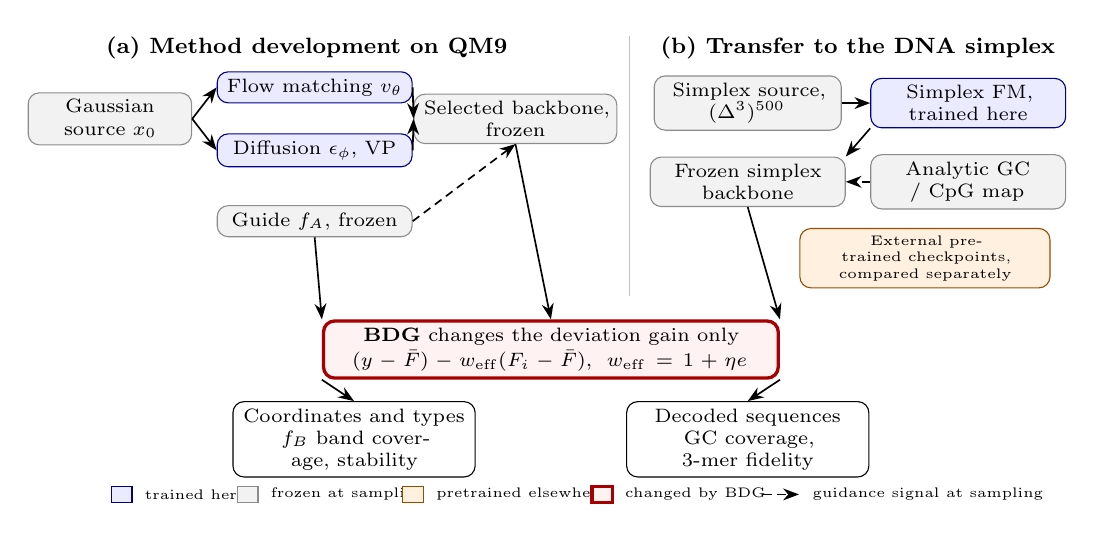
\begin{tikzpicture}[font=\scriptsize,
  box/.style={draw,rounded corners,align=center,inner sep=2.5pt},
  trained/.style={box,fill=blue!8,draw=blue!55!black},
  frozen/.style={box,fill=black!5,draw=black!45},
  pre/.style={box,fill=orange!12,draw=orange!60!black},
  innov/.style={box,fill=red!5,draw=red!65!black,very thick},
  arr/.style={-{Stealth},semithick},
  gsig/.style={-{Stealth},semithick,densely dashed},
  key/.style={draw,minimum width=0.26cm,minimum height=0.2cm,inner sep=0}]

% ---- panel (a) : development on QM9
\node[font=\footnotesize\bfseries] at (0.3,2.05) {(a) Method development on QM9};
\node[frozen,text width=1.9cm] (src) at (-2.2,1.15) {Gaussian source $x_0$};
\node[trained,text width=2.3cm] (fm)  at (0.4,1.55) {Flow matching $v_\theta$};
\node[trained,text width=2.3cm] (vp)  at (0.4,0.75) {Diffusion $\epsilon_\phi$, VP};
\node[frozen,text width=2.4cm] (sel)  at (2.95,1.15) {Selected backbone,\\frozen};
\node[frozen,text width=2.3cm] (guide) at (0.4,-0.15) {Guide $f_A$, frozen};
\draw[arr] (src.east)--(fm.west);
\draw[arr] (src.east)--(vp.west);
\draw[arr] (fm.east)--(sel.west);
\draw[arr] (vp.east)--(sel.west);
\draw[gsig] (guide.east)--(sel.south);

% ---- divider
\draw[black!25] (4.4,2.2)--(4.4,-1.1);

% ---- panel (b) : transfer to the simplex
\node[font=\footnotesize\bfseries] at (7.3,2.05) {(b) Transfer to the DNA simplex};
\node[frozen,text width=2.2cm] (src2)  at (5.9,1.35) {Simplex source, $(\Delta^3)^{500}$};
\node[trained,text width=2.3cm] (sfm)   at (8.7,1.35) {Simplex FM, trained here};
\node[frozen,text width=2.3cm] (sel2)  at (5.9,0.35) {Frozen simplex\\backbone};
\node[frozen,text width=2.3cm] (prop2) at (8.7,0.35) {Analytic GC / CpG map};
\draw[arr] (src2.east)--(sfm.west);
\draw[arr] (sfm.south west)--(sel2.north east);
\draw[gsig] (prop2.west)--(sel2.east);
\node[pre,text width=3.0cm,font=\tiny] (ext) at (8.15,-0.62)
  {External pretrained checkpoints,\\compared separately};

% ---- the shared rule
\node[innov,text width=5.6cm] (bdg) at (3.4,-1.78)
  {\textbf{BDG} changes the deviation gain only\\[1pt]
   $(y-\Fbar)-\weff(F_i-\Fbar)$, \ $\weff=1+\eta e$};
\draw[arr] (guide.south)--(bdg.north west);
\draw[arr] (sel.south)--(bdg.north);
\draw[arr] (sel2.south)--(bdg.north east);

% ---- outputs
\node[box,text width=2.9cm] (o1) at (0.9,-2.92) {Coordinates and types\\$f_B$ band coverage, stability};
\node[box,text width=2.9cm] (o2) at (5.9,-2.92) {Decoded sequences\\GC coverage, 3-mer fidelity};
\draw[arr] (bdg.south west)--(o1.north);
\draw[arr] (bdg.south east)--(o2.north);

% ---- key
\node[key,fill=blue!8,draw=blue!55!black] at (-2.05,-3.62) {};
\node[anchor=west,font=\tiny] at (-1.88,-3.62) {trained here};
\node[key,fill=black!5,draw=black!45] at (-0.45,-3.62) {};
\node[anchor=west,font=\tiny] at (-0.28,-3.62) {frozen at sampling};
\node[key,fill=orange!12,draw=orange!60!black] at (1.65,-3.62) {};
\node[anchor=west,font=\tiny] at (1.82,-3.62) {pretrained elsewhere};
\node[key,fill=red!5,draw=red!65!black,very thick] at (4.05,-3.62) {};
\node[anchor=west,font=\tiny] at (4.22,-3.62) {changed by BDG};
\draw[gsig] (6.1,-3.62)--(6.55,-3.62);
\node[anchor=west,font=\tiny] at (6.6,-3.62) {guidance signal at sampling};
\end{tikzpicture}
\caption{Overview of the study. \textbf{(a)} QM9: the two families we train, the frozen backbone, and the frozen guide supplying the property gradient (dashed). \textbf{(b)} Transfer to the simplex. External checkpoints are never pooled with models trained here.}
\label{fig:overview}
\end{figure}

\section{Results}
\subsection{Evaluation Protocol}\label{sec:protocol}
\subsubsection{Metrics}
Every target is the \textbf{q50} value, the median of that property's training distribution, for all five properties across both modalities; no other quantile is run. Bold marks our method in every table; no value is bolded as largest. On QM9, controllability is band coverage $\IB$, the decoded fraction within $\delta=2\operatorname{MAE}_{\mathrm{cal}}(f_B)$ of that target (Appendix~\ref{app:evaluation}); fidelity and diversity are molecule stability, RDKit validity, uniqueness and distinct-valid yield. On the DNA simplex it is GC-band coverage under the exact count, with 3-mer fidelity and pairwise distinctness (Appendix~\ref{app:m2}).

\subsubsection{Fair Comparison and Computational Budget}
The operator chose $n{=}2{,}000$ per cell in batches of 500 over three seeds, against the pre-registered power table. The run cost $81.2$ GPU-hours; settings, hardware and the cost split are in Appendices~\ref{app:training} and~\ref{app:evaluation}. Two mismatches remain: equal $w$ is equal nominal strength, not equal applied force, and external checkpoints stay inside their own generator (Table~\ref{tab:backends}).

\subsubsection{Statistical Reporting}
Each cell pools its three seeds, so every fraction rests on $6{,}000$ samples and its standard error is binomial. A contrast between two arms is reported unpaired, $\mathrm{se}=\sqrt{\mathrm{se}_a^2+\mathrm{se}_b^2}$, which is conservative by about $\sqrt2$ because arms in a cell share their initial noise, molecule sizes, target and band. Verdicts are called at the pre-registered Bonferroni bar $z{=}2.99$, $\alpha{=}0.05$ over eighteen contrasts, two-sided; at this $n$ the smallest resolvable difference in coverage is $1.56$ points, so a null is reported beside that figure and not as an absence of effect. No chemistry floor governs the protocol, and the consequence travels with every number: a coverage leaderboard would crown whichever arm destroyed the most chemistry, so coverage is always printed beside the stability it cost. Produced numbers are labelled separately from quoted ones.

\subsection{Modality 1: Flow Matching versus Diffusion}\label{sec:fmvd}
\textbf{We did not select a backbone on evidence.} The matched flow-against-diffusion comparison was cancelled before it produced a usable cell, so we report guidance on the three generators we could run (Table~\ref{tab:fmvd}), never pooled; the external diffusion checkpoint is not a substitute for it.

\begin{table}[!htbp]
\centering\small
\caption{QM9 generators under one sampler, evaluator, size draw and card, as seed mean $\pm$ sd over three seeds of $n{=}2{,}000$. The borrowed rows are \emph{not} matched to ours in data, architecture, parameters or budget. NFE includes terminal denoising.}
\label{tab:fmvd}
\begin{tabular}{lccccc}
\toprule
Generator & Mol. stab.$\uparrow$ & Validity$\uparrow$ & Uniq.$\uparrow$ & NFE$\downarrow$ & s/sample$\downarrow$\\
\midrule
Flow matching, ours ($3.75$\,M) & $0.3970${\tiny$\pm.0061$} & $0.7562${\tiny$\pm.0108$} & $0.9985$ & $100$ & $0.051$\\
\midrule
EquiFM, borrowed ($5.34$\,M) & $0.8622${\tiny$\pm.0032$} & $0.9377${\tiny$\pm.0060$} & $0.9972$ & $100$ & $0.086$\\
EDMsecond, borrowed ($5.34$\,M) & $0.6715${\tiny$\pm.0125$} & $0.8602${\tiny$\pm.0128$} & $0.9977$ & $101$ & $0.087$\\
\bottomrule
\end{tabular}
\end{table}


\subsection{Modality 1: Guided versus Unguided Generation}\label{sec:guidworks}
Guidance raises decoded coverage in 8 of 9 generator and property pairs, paid for in chemistry (Table~\ref{tab:guidance}). At the bar it clears in only 5 of those 9, failing on $\alpha$ throughout and on EquiFM's gap, at a cost of $3.96$ points of molecule stability over the six matched cells.

\begin{table}[!htbp]
\centering\small
\caption{Guidance against a matched unguided control on our flow model at the q50 target, $w{=}1$, $n{=}2{,}000\times3$ seeds. Cells are $\mu$\,/\,$\alpha$\,/\,gap; DV is distinct-valid molecules per attempt. The strength axis exists only in the ablation (Table~\ref{tab:ablation}).}
\label{tab:guidance}
\begin{tabular}{lcccc}
\toprule
Arm & IB$\uparrow$ & Mol. stab.$\uparrow$ & Validity$\uparrow$ & DV$\uparrow$\\
\midrule
Unguided & $.078$\,/\,$.050$\,/\,$.103$ & $.397$\,/\,$.397$\,/\,$.397$ & $.756$\,/\,$.756$\,/\,$.756$ & $.755$\,/\,$.755$\,/\,$.755$\\
Plug-in & $.106$\,/\,$.061$\,/\,$.126$ & $.356$\,/\,$.372$\,/\,$.336$ & $.725$\,/\,$.737$\,/\,$.699$ & $.724$\,/\,$.736$\,/\,$.698$\\
\bottomrule
\end{tabular}
\end{table}


\subsection{Modality 1: Innovation Ablations}\label{sec:ablations}
The mechanism is isolated here, because $w$ is held fixed along every row (Table~\ref{tab:ablation}). Coverage tracks the \emph{measured} deviation gain $\weff$, at Spearman $0.92$ to $0.99$ in all twelve grids. The contracting row raises coverage in 5 of 12 grids, four at $w{=}1$; the expanding row lowers it in 12 of 12, clearing the bar in 11, and widens the batch past unguided, $R$ $1.15$ to $1.25$, in 6 of 6 cells. That last is an operating point no strength reaches: at $w{=}4$ the strength dial still only narrows. Appendix~\ref{app:evaluation} prices the two dials against each other. Three controls did not run, a one-sided residual, an open-loop replay and a signed-strength plug-in, and without the replay the grid cannot show the \emph{feedback} is necessary.

\begin{table}[!htbp]
\centering\small
\caption{The registered grid: $\eta\in\{1,2,4,8\}\times\tau_{\mathrm{mult}}\in\{0.5,0.75,1,1.5\}$ at $w\in\{1,4\}$, two generators, three properties, three seeds, 612 cells. Each result is the unpaired change against the $\eta{=}0$ cell.}
\label{tab:ablation}
\begin{tabular}{llc}
\toprule
Control & What it isolates & Result over 12 grids\\
\midrule
$\eta=0$ against plug-in & the identity & bit-exact on ours; $4\times10^{-3}$ on EquiFM\\
IB against measured $\weff$ & dispersion, not strength & Spearman $0.92$--$0.99$, 12 of 12\\
$\tau_{\mathrm{mult}}{=}0.5$, $\eta$ rising & contraction & IB rises in 5 of 12, four at $w{=}1$\\
$\tau_{\mathrm{mult}}{=}1.5$, $\eta$ rising & expansion & IB falls in 12 of 12, 11 past the bar\\
\bottomrule
\end{tabular}
\end{table}


\subsection{Modality 1: Comparison with Recent Methods}\label{sec:recent}
\textbf{BDG does not beat the arm it is built on} (Table~\ref{tab:recent}). Against plug-in, which is BDG at $\eta{=}0$, the twelve contrasts of two setpoints over three properties and two generators give no gain at the bar, three losses and nine ties. \textbf{TFG leads coverage in 5 of 6 cells}, and by a wide margin, while spending 8 to 27 points of molecule stability to do it. Coverage alone would therefore rank TFG first and say nothing useful, which is why every coverage figure here is printed beside the chemistry it cost.

\begin{table}[!htbp]
\centering\small
\caption{Guidance rules on our frozen flow model, $w{=}1$, $n{=}2{,}000\times3$ seeds, cells $\mu$\,/\,$\alpha$\,/\,gap. Prior-method rows are our adaptations (Appendix~\ref{app:comparisons}); both registered BDG setpoints are shown.}
\label{tab:recent}
\begin{tabular}{lcc}
\toprule
Method & IB$\uparrow$ & Mol. stab.$\uparrow$\\
\midrule
Unguided, internal reference & $.078$\,/\,$.050$\,/\,$.103$ & $.397$\,/\,$.397$\,/\,$.397$\\
\midrule
DPS-style plug-in \citep{chung2023dps} & $.106$\,/\,$.061$\,/\,$.126$ & $.356$\,/\,$.372$\,/\,$.336$\\
TMPD-inspired \citep{boys2024tmpd} & $.090$\,/\,$.061$\,/\,$.116$ & $.384$\,/\,$.389$\,/\,$.373$\\
LGD-MC \citep{song2023lgd} & $.096$\,/\,$.052$\,/\,$.108$ & $.399$\,/\,$.392$\,/\,$.395$\\
TFG \citep{ye2024tfg} & $.288$\,/\,$.105$\,/\,$.275$ & $.245$\,/\,$.268$\,/\,$.144$\\
\midrule
\textbf{BDG, $\tau_{\mathrm{mult}}{=}0.5$ (ours)} & $.112$\,/\,$.070$\,/\,$.142$ & $.351$\,/\,$.364$\,/\,$.300$\\
\textbf{BDG, $\tau_{\mathrm{mult}}{=}1$ (ours)} & $.089$\,/\,$.056$\,/\,$.106$ & $.405$\,/\,$.379$\,/\,$.376$\\
\bottomrule
\end{tabular}
\end{table}


\subsection{Modality 2: Transfer of the Innovation}\label{sec:m2}
The rule transfers in its dispersion term (Table~\ref{tab:m2}). At $w{=}1$ the gain over plug-in is $0.42$ points on GC, below the $1.89$ this $n$ resolves, but $4.82$ on CpG, which clears it; at $w{=}4$ it is $2.32$ on GC and $16.8$ on CpG. At fixed strength the gain sweep repeats: raising $\eta$ from 0 to 8 at $\tau_{\mathrm{mult}}{=}0.5$ moves coverage from $+0.15$ to $+4.23$ points, and inverting the setpoint reverses the sign to $-0.40$. One caveat dominates: the guidance window matters more than the rule, since opening it to $t\ge0$ buys plug-in $22.8$ points, about five times the best obtained inside the window (Appendix~\ref{app:m2}).

\begin{table}[!htbp]
\centering\small
\caption{DeepFlyBrain at $L{=}500$, GC band, $n{=}2{,}000\times3$ seeds, window $t\ge0.5$. JSD is 3-mer mismatch and diversity mean pairwise Hamming distance, both at $w{=}1$; the diversity ceiling is $0.747$. A dash marks a comparator we did not run.}
\label{tab:m2}
\begin{tabular}{lcccc}
\toprule
Method & IB, $w{=}1$$\uparrow$ & IB, $w{=}4$$\uparrow$ & JSD$\downarrow$ & Diversity$\uparrow$\\
\midrule
Simplex FM, unguided & $0.1395$ & $-$ & $0.00045$ & $0.7456$\\
Simplex FM $+$ plug-in & $0.1403$ & $0.1410$ & $0.00045$ & $0.7456$\\
\textbf{Simplex FM $+$ BDG, $\tau_{\mathrm{mult}}{=}0.5$} & $0.1445$ & $0.1642$ & $0.00049$ & $0.7456$\\
\textbf{Simplex FM $+$ BDG, $\tau_{\mathrm{mult}}{=}1$} & $0.1402$ & $0.1407$ & $0.00045$ & $0.7456$\\
\midrule
Dirichlet FM, Fisher Flow, MOG-DFM \citep{stark2024dirichlet,davis2024fisher,chen2025multi} & $-$ & $-$ & $-$ & $-$\\
\bottomrule
\end{tabular}
\end{table}


\subsection{Cross-Modality Analysis and Failure Modes}\label{sec:failure}
The residual acts through the contraction term in both state spaces, and in neither does it buy coverage over the arm it modifies. Two confounds bound the result: the arms that gain most clip most, and the borrowed generator's sampler is not deterministic, so its re-runs move coverage by as much as the effect measured on it.

\section{Discussion}
Guidance works and is paid for in chemistry, and the dispersion residual behaves as derived without converting that into coverage. The ablation is causal within its design; the headline comparison is not.

Equation~\eqref{eq:bdg} accounts for the null: BDG reaches nothing outside the plug-in field's two-parameter family, and what predicts coverage is the realised gain $\weff$, not the setpoint.

Three limitations bound the claim. A held-out predictor scores coverage, so an arm can gain by exploiting it; a second evaluator already changes 11 of 84 verdicts, and a third at a common band would settle that. The grid cannot separate feedback from schedule, which the open-loop replay would settle. And the borrowed generator's sampler is non-deterministic, so its re-runs move coverage by as much as the effects measured on it. The narrowest claim supported is that the setpoint reaches spread states no strength setting reaches, without improving coverage over the rule it modifies.
% MAIN_TEXT_END
\clearpage
\bibliographystyle{ieeetr}
\bibliography{citation,refs_extra}
\clearpage
\appendix
\renewcommand{\thetable}{S\arabic{table}}
\setcounter{table}{0}
\renewcommand{\thefigure}{S\arabic{figure}}
\setcounter{figure}{0}
\section{Reproducibility and Extended Protocol}
\subsection{Data Sources and Splits}\label{app:data}
The QM9 source is the DeepChem/MoleculeNet packaging. The project retains the 3{,}054 entries removed as uncharacterized in common EDM preprocessing, so its data definition differs from those benchmarks. A seeded permutation creates the splits: 51{,}527 molecules in \texttt{train\_a}, a disjoint 51{,}527 in \texttt{train\_b}, 17{,}748 validation and 13{,}083 test. Centering removes translation; predictors are invariant. Coordinates and one-hot types have no additional scaling. Predictors use training-derived property normalization. Molecular sizes are paired across arms within each backend.

DeepFlyBrain is stored in \path{proj1/m2/blade_bundle/dfb500.npz}. Four ambiguous training examples were excluded from the supplied 83{,}726. The channel order is A/C/G/T and length is 500, and the retained train/validation/test counts are 83{,}722/10{,}505/10{,}434. Cell-type labels are not supplied to our unconditional generator. Random-example splits do not establish sequence-cluster or out-of-distribution generalization. The older 200-base-pair Kenyon-cell setup is excluded from the final comparison.

\subsection{Training and Checkpoint Records}\label{app:training}
Table~\ref{tab:training} separates configurations from final provenance. Matching configurations does not establish equal completed training. Checkpoints, actual epochs, and selection rules must accompany FM--VP evaluation. The existing FM record uses final EMA weights; VP code selects by validation generation stability with loss as tie-breaker. This difference must be disclosed or aligned before selection.

\begin{table}[!htbp]
\centering\small
\caption{Training configuration and recorded properties. Asterisks mark configured settings requiring final run verification. P denotes missing final provenance. Predictor counts are per property network.}
\label{tab:training}
\begin{tabular}{llll}
\toprule
Setting & Molecular FM / VP & $f_A$ / $f_B$ & Sequence FM\\
\midrule
Architecture & EGNN, 256, 8 layers & invariant EGNN, 128, 4 & CNN, 128, 10 layers\\
Parameters & 3.75 M each & 429{,}825 each & approximately 1.02 M\\
Training split & \texttt{train\_a} & \texttt{train\_a} / \texttt{train\_b} & DeepFlyBrain train\\
Objective & velocity / noise MSE & property MSE & velocity MSE\\
Epochs & 1{,}500$^*$ & 120 & 1{,}500 recorded\\
Batch & 256$^*$ & 128 & 256\\
Optimizer & Adam$^*$ & Adam & \pend\\
Learning rate & $2\times10^{-4}$, cosine$^*$ & $3\times10^{-4}$, cosine & $2\times10^{-3}$, cosine\\
EMA & 0.9999$^*$ & none & \pend\\
Run seed & 20260918$^*$ & \pend & \pend\\
Hashes / hardware & \pend & \pend & \pend\\
\bottomrule
\end{tabular}
\end{table}

For coordinates $c$ and features $f$, the norm in Equations~\eqref{eq:fm} and~\eqref{eq:vp} is
\[
\|z\|_M^2=\frac{\|M\odot z^c\|_2^2}{3\sum M}+\frac{\|M\odot z^f\|_2^2}{5\sum M}.
\]
The mask $M$ broadcasts over channels. Coordinate noise is projected to zero center of mass, giving dimension $3(N-1)$ for $N$ atoms. Feature noise is Gaussian. Atom types use the largest final feature component. VP time $u$ is clean-to-noise; flow time $t$ is noise-to-data.

The VP process and loss of Section~\ref{sec:diff} are
\begin{equation}
\begin{aligned}
x_u&=a(u)x_1+\sigma(u)\epsilon,\quad a(u)=e^{-\frac12(0.1u+9.95u^2)},\quad \sigma^2=1-a^2,\\
\mathcal L_{\mathrm{VP}}&=\mathbb E\|\epsilon_\phi(x_u,u;M)-\epsilon\|_M^2,
\end{aligned}
\label{eq:vp}
\end{equation}
with $\beta(u)=0.1+19.9u$ and probability-flow ODE $\mathrm dx/\mathrm du=-\tfrac12\beta(u)(x+s_\phi)$, where $s_\phi=-\epsilon_\phi/\sigma$. QM9 preprocessing keeps coordinates and one-hot types unscaled, and the dataset supplies 133{,}885 molecules before splitting.

\subsection{Evaluation and Cost Accounting}\label{app:evaluation}
Pricing the two dials against each other on the ablation grid, in coverage points gained per point of molecule stability lost against the same $\eta{=}0$, $w{=}1$ cell: on our generator the setpoint buys $0.52$ to $0.81$ against the strength dial's $0.38$ to $0.53$, so it is the cheaper dial there; on the borrowed generator the two are indistinguishable ($0.06$ to $0.39$ against $0.08$ to $0.37$). The molecular protocol fixes seeds 20261001, 20261002, and 20261003, q50 targets, $w=1$, $t_{\min}=0.5$, and batch 500. Per-cell $n$ was 2{,}000, run as four separately coupled batches of 500, so each reported fraction pools $3n=6{,}000$ samples over the three seeds. Increasing $n$ adds batches without changing each variance estimator's sample count. Batch size is a BDG design parameter. Band coverage is $\IB=n^{-1}\sum_i\mathbf1\{|f_B(\hat x_i)-y|\le\delta\}$ over decoded samples, with $\delta=2\operatorname{MAE}_{\mathrm{cal}}(f_B)$; it inherits $f_B$'s error, so a guided arm can raise it by exploiting the evaluator.

The calibration pool contains 3{,}000 molecules from the two training halves. Internal predictors are calibrated only on the half they did not train on. Evaluator-specific acceptance widths differ from $\tau=\tau_{\mathrm{mult}}f_A.\texttt{y\_std}$. Cells record widths and predictor identities (Table~\ref{tab:backends}).

\begin{table}[!htbp]
\centering\small
\caption{Molecular guidance backends. External generators are pretrained and frozen. Results stay within backend. External EDM is separate from our trained VP comparison.}
\label{tab:backends}
\begin{tabular}{lll}
\toprule
Generator & Guide / evaluator & Headline arms\\
\midrule
Our FM & internal disjoint pair & all seven\\
External EquiFM & released TFG pair & all seven\\
External EDMsecond & internal disjoint pair & unguided, plug-in\\
\bottomrule
\end{tabular}
\end{table}

The seven arms are unguided, plug-in, TMPD-inspired, LGD-MC, TFG, and BDG at $\eta=4$, $\tau_{\mathrm{mult}}\in\{0.5,1\}$. The registered ablation grid is $\eta\in\{1,2,4,8\}$ and $\tau_{\mathrm{mult}}\in\{0.5,0.75,1,1.5\}$, with one $\eta=0$ setting, at $w\in\{1,4\}$. Two setpoints cannot establish a monotone curve; the ablation supplies additional gains and setpoints. All arms remain visible regardless of stability. The pilot chemistry floor does not govern this protocol.

Atom stability is the fraction satisfying the project's bond/valence rules; molecule stability requires all atoms to pass. RDKit validity uses fixed reconstruction and sanitization. Uniqueness divides distinct canonical SMILES by valid samples; distinct-valid yield divides distinct valid molecules by all attempts. Stability and validity are bond-table conventions, not energies, and uniqueness saturates near one at this scale. We report attempted, decoded, valid, and distinct-valid counts, and every guided arm reports the metric guidance optimises beside one it does not. Band coverage includes chemically invalid samples and cannot alone measure usable yield, so every coverage figure is printed beside the stability and validity it cost.

We distinguish $f_A$ endpoint spread as a controller diagnostic from $f_B$ decoded spread as an evaluation diagnostic. Neither equals structural diversity. The analysis reports three seed values, mean, sample standard deviation, and paired changes under common noise. Intervals respect coupled batches. Sampling seeds quantify sampling variation at fixed weights, not training-seed uncertainty.

Cost accounting covers generator forwards, generator vector--Jacobian products, guide forwards/backwards, peak memory, and seconds per sample on matched hardware. BDG adds reductions to plug-in's calls; equal calls do not establish equal runtime. The reported run cost $81.2$ GPU-hours on one card type, $16.0$ for the headline stage and $65.2$ for the larger ablation.

\subsection{Baseline Adaptations and Comparison Limits}\label{app:comparisons}
Our DPS-style plug-in adapts inverse-problem guidance to a Gaussian property energy and flow endpoint. TMPD-inspired guidance linearizes property uncertainty. LGD-MC and TFG also require disclosed endpoint, noise, and sampler choices. These adaptations do not reproduce every published benchmark.

External EquiFM and EDMsecond differ from our FM--VP pair in data, architecture, and parameterization. EquiFM uses TFG predictors with different acceptance widths and uncertain training overlap. Coverage comparisons stay within backend and predictor pair.

Dirichlet FM, Fisher Flow, and MOG-DFM require common length, target, band width, conditioning, decoding, and reference data. Published class-conditioned scores do not establish GC/CpG-band performance. These three comparisons did not run. Guidance ports on our sequence generator do not themselves reproduce these three models.

\subsection{Sequence Transfer Protocol}\label{app:m2}
The shipped model is \path{proj1/m2/blade_bundle/fm_m2_dfb500.pt}. Its path joins a uniform Dirichlet source to one-hot sequences. The sampler clamps each Euler update to nonnegative values, renormalizes per position, and decodes by $\arg\max$. Endpoint extrapolation used by the guide need not lie on the simplex, creating a possible mismatch with decoded counts.

For relaxed sequence $p\in\mathbb R^{L\times4}$,
\[
F_{\mathrm{GC}}(p)=L^{-1}\sum_{j=1}^L(p_{j,C}+p_{j,G}),\qquad
F_{\mathrm{CpG}}(p)=(L-1)^{-1}\sum_{j=1}^{L-1}p_{j,C}p_{j+1,G}.
\]
GC is affine; CpG is quadratic. Evaluation counts bases or adjacent pairs after decoding. Exact counts have no prediction error to define a nonzero band. Existing code uses $\delta=\max(0.16s,4.4/(L-1))$, with training-property standard deviation $s$. GC/CpG counting increments are $1/L$ and $1/(L-1)$; the current floor uses the latter for both. Final widths must be fixed before comparison and are not commensurate with molecular bands.

The sequence protocol is $n=2{,}000$ per cell in batches of 500 over three seeds, and every shipped sequence cell used $t_{\min}=0.5$; the driver's $t_{\min}=0$ default was not used. Opening the window to $t\ge0$ raises plug-in coverage by $22.8$ points, but it also saturates the trust region on about a third of steps, which collapses the arms onto one another. Comparator alignment for the three external rows remains unsettled.

Three-mer JSD compares generated and held-out frequencies. Diversity is mean normalized pairwise Hamming distance, with the pair-sampling rule recorded. Evaluation will also include decoding confidence and duplicates. Composition statistics do not establish enhancer activity or cell-type specificity.

\subsection{BDG Algorithm and Algebraic Limits}\label{app:algebra}
Algorithm~\ref{alg:bdg} gives the update. All weights are fixed. Batch statistics determine coefficients; the pullback differentiates properties with coefficients held fixed. Differentiating a loss through the coefficients would produce another update.

\begin{algorithm}[htbp]
\caption{One BDG-guided Euler step}\label{alg:bdg}
\begin{algorithmic}[1]
\Require batch $x_t$, frozen $v_\theta$ and $f$, target $y$, scale $s>0$, gain $\eta\ge0$, setpoint $\tau>0$, strength $w$, step $h$, start $t_{\min}$
\State $v\gets v_\theta(x_t,t;M)$
\If{$t<t_{\min}$} \State \Return $\Pi(x_t+h v)$ \EndIf
\State $m\gets x_t+(1-t)v_\theta(x_t,t;M)$ with gradients enabled
\State $F_i\gets f(m_i)$; $\Fbar\gets B^{-1}\sum_iF_i$
\State $\Vb\gets (B-1)^{-1}\sum_i(F_i-\Fbar)^2$ if $B>1$, else $\tau^2$
\State $e\gets(\Vb-\tau^2)/\tau^2$ \Comment{one-sided: $e\gets\max(e,0)$}
\State $a_i\gets\sg\{[(y-F_i)-\eta e(F_i-\Fbar)]/s^2\}$
\State $G\gets\operatorname{VJP}_{x_t}(F,a)$
\State $C_i\gets w(1-t)/\max(t,\varepsilon)\,G_i$
\State $C_i\gets C_i\min(1,\|v_i\|/\max(\|C_i\|,\varepsilon))$
\State \Return $\Pi\{x_t+h(v+C)\}$
\end{algorithmic}
\end{algorithm}

For molecules, $\Pi$ applies masks and coordinate centering; for sequences it clamps and renormalizes. The numerical guard $\varepsilon$ is implementation-specific. The sequence score factor uses $10^{-6}$. At $B=1$, $F_i-\Fbar=0$ and dispersion vanishes even though the sequence code records a different variance fallback.

The bound $\weff\ge1-\eta$ follows from $\Vb\ge0$. Positive $e$ strengthens contraction and negative $e$ weakens it, so the widening condition $\weff<0$ requires $\eta>1$ and $\Vb<\tau^2(1-1/\eta)$. For $\weff\ne0$, Equation~\eqref{eq:bdg} reads $n_i=\weff(y_{\mathrm{eff}}-F_i)$ with effective target $y_{\mathrm{eff}}=(y+\eta e\Fbar)/\weff$; at $\weff=0$ it remains finite. In the simplified property ODE $\dot F_i=(y-\Fbar)-\weff(F_i-\Fbar)$, $\dot V_b=-2\weff V_b$. For $\eta>1$, a positive stationary variance is $\tau^2(1-1/\eta)$, below the setpoint. This assumes homogeneous unit response, continuous time, and no generator drift, clipping, or projection. It gives no convergence guarantee for the implemented sampler.

\clearpage
\subsection{Implementation Map and Pending Evidence}\label{app:implementation}
Table~\ref{tab:provenance} connects the paper to the repository. Archived pilots remain available. No pilot effect substitutes for one of the experiments that did not run.

\begin{table}[!htbp]
\centering\small
\caption{Source and evidence map, relative to the repository root.}
\label{tab:provenance}
\begin{tabular}{ll}
\toprule
Component & Source or protocol\\
\midrule
Molecular BDG & \path{proj1/src/guidance.py}, \texttt{mode == "bdg"}\\
Integration & \path{proj1/src/sampling.py}\\
VP training & \path{proj1/scripts/train_diffusion.py}\\
Final molecular sweep & \path{proj1/scripts/transfer_sweep.py}\\
Headline protocol & \path{docs/protocol/FULL_RUN_V3_PROTOCOL.md}\\
Ablation protocol & \path{docs/protocol/ABLATION_V3_PROTOCOL.md}\\
Sequence implementation & \path{proj1/m2/m2_sweep.py}\\
Sequence protocol status & \path{docs/protocol/MODALITY2_V3_PLAN.md}\\
Algebraic checks & \path{proj1/tests/test_bdg.py}\\
\bottomrule
\end{tabular}
\end{table}

\textbf{Run identity.} Each final result requires a generator checkpoint hash,
guide and evaluator identities, dataset/split identifiers, target and band width,
sample count, batch size, seed, integrator, step count, guidance window, nominal
strength, and method-specific settings. BDG additionally requires its gain,
setpoint multiplier, one-sided flag, and any replay schedule. A common method
name is insufficient to identify a matched comparison.

\textbf{Evidence status.} Implementation and algebraic checks address whether the
specified update is computed; they do not establish a coverage improvement,
sample-quality advantage, or successful transfer. The empirical evidence in
Section~\ref{sec:ablations} onward comes from the declared comparison protocol
with per-seed measurements. Older pilot outputs remain separate because their
targets, strengths, batch sizes, or sample counts can differ.

\textbf{Reproducibility record.} The release pairs each aggregate with its
underlying cell records and analysis configuration. Hardware, software versions,
wall-clock costs, and peak memory accompany the neural-call counts.
Configuration changes and failed or excluded runs require explicit records.
Identifiers come from the run manifests and are not reconstructed from this
draft's table structure.


\end{document}
